\documentclass[aps,prd,twocolumn,10pt,superscriptaddress,nofootinbib,longbibliography,floatfix]{revtex4-2}

\usepackage{amsmath,amssymb,amsfonts}
\usepackage{bm}
\usepackage{graphicx}
\usepackage{booktabs}
\usepackage{xcolor}
\usepackage{hyperref}
\graphicspath{{figures/}}
\hypersetup{colorlinks=true,linkcolor=blue,citecolor=blue,urlcolor=blue}

\newcommand{\dd}{\mathrm{d}}
\newcommand{\Ham}{\mathcal{H}}
\newcommand{\Mom}{\mathcal{M}}

\begin{document}

\title{Collisionless collapse to primordial black holes in an early matter era:\\ Scope, set-up, and first tests (working note v0)}

\author{Track A of the numerical-relativity particle-in-cell cosmology program}

\date{Working note v0, state of 15 November 2026}

\begin{abstract}
In an early era dominated by pressureless matter every overdensity grows until it collapses, and whether the collapse ends in a black hole is decided by what can halt it first: departures from spherical symmetry, velocity dispersion, angular momentum, or the end of the era. The analytic estimates of this threshold disagree with one another, and the one calculation with particles in full general relativity finds black holes an order of magnitude below the estimate from the hoop conjecture. This working note scopes a program that computes the threshold, the mass, the spin and the gravitational waves of these black holes with a particle-in-cell method coupled to numerical relativity, converged in particle number, cell size and domain size. It fixes a definition of the threshold for collisionless matter before any run, sets up an expanding ball with an exact interior solution for verification and a periodic box with the data of the earlier calculation for the threshold line, and records the tests done so far. The initial data satisfy the constraints at the order of the finite differences that check them; two independent constructions of the data, two readers of their tables and three solutions of the exact evolution agree to rounding error; the analytic criteria, coded from their papers, reproduce the published values and spread over two orders of magnitude in the predicted threshold. The first runs in full general relativity are specified with predicted times of turnaround, trapping and crunch, and are waiting for computing time.
\end{abstract}

\maketitle

\section{Introduction}\label{sec:intro}

A universe dominated by pressureless matter has no Jeans length. A spherical overdensity of uniform density therefore collapses to a black hole whatever its amplitude \cite{Ebrahimian:2025md}, and the formation of primordial black holes in an early matter era becomes a question about what stops the collapse before the matter is inside its gravitational radius. Generic overdensities are triaxial and flatten first along one axis into a pancake; inside the pancake the matter streams cross, its velocity dispersion grows, and tidal torques give it angular momentum. Each of these effects can halt the collapse in a virialized halo, and so can the end of the matter era itself. The calculation is a strong-field problem with crossing streams of collisionless matter, which a fluid description follows only up to the first crossing.

The analytic estimates rest on different halting mechanisms: the hoop conjecture applied to the Zel'dovich pancake \cite{Harada:2016hoop}, the Kerr bound on the spin acquired by tidal torques \cite{Harada:2017spin}, the crossing time of a velocity dispersion \cite{Harada:2022disp}, and the profile and peak statistics of the overdensity \cite{Ebrahimian:2025md,Ye:2025md}. Full numerical relativity has followed scalar-field proxies through collapse and accretion \cite{deJong:2021nr,deJong:2023spin}, and the choice of slicing changes the outcome of dust collapse \cite{Munoz:2026gauge}. The one calculation with collisionless particles in full general relativity, by Yoo, Escriv\`a, Harada and Kohri \cite{Yoo:2026mdpbh}, finds apparent horizons at one ellipticity for amplitudes an order of magnitude below the Zel'dovich-hoop estimate, from runs at a single resolution, without horizon masses, spins or waveforms.

The numerical-relativity particle-in-cell method of Wu and Most \cite{Wu:2026nrpic} couples macroparticles on geodesics to the Z4c evolution of the spacetime on an adaptive mesh, with moving punctures and an apparent-horizon finder. It can continue a collapse past horizon formation, follow accretion, measure the mass and spin of the black hole and extract its waveform, and it can be run at several particle numbers and cell sizes. This program applies a version of that method, rebuilt for isolated systems and extended to periodic expanding domains in the code AthenaK, to the matter-era threshold. The work is carried out by large-language-model agents under human direction.

This note records the scoping stage. Section~\ref{sec:problem} states the problem, a definition of the threshold fixed before any run, and what the estimates predict. Section~\ref{sec:setup} gives the two set-ups and the numerical methods. Section~\ref{sec:tests} reports the tests done so far, and Sec.~\ref{sec:plan} the plan to the next gates and what is open. Table~\ref{tab:parameters} holds the parameters, and Table~\ref{tab:ledger} every number of the note with the registered run that produced it.

\section{The threshold problem}\label{sec:problem}

\subsection{Amplitude and shape}\label{sec:amplitude}

For the comparison with Ref.~\cite{Yoo:2026mdpbh} the overdensity is the curvature peak of that work, a Gaussian in the logarithm of the conformal factor with amplitude $\mu$, wavenumber $k$, ellipticity $e$ and prolateness $p$,
\begin{equation}\label{eq:profile}
\begin{split}
\ln\Psi = \frac{\mu}{2}\, e^{-k^2 r^2/6}\Big[1&+\frac{k^2}{6}\,p\,(2X^2-Y^2-Z^2)\\
&+\frac{k^2}{2}\,e\,(Y^2-Z^2)\Big],
\end{split}
\end{equation}
with Cartesian coordinates $X,Y,Z$ and $r^2=X^2+Y^2+Z^2$. Two measures of the amplitude are in use: the linear central density contrast $\delta_c$ at horizon entry, the epoch at which the comoving compaction radius $r_m$ equals the Hubble radius, and the linear mean contrast $\bar\delta_{\rm ent}$ inside $r_m$ at the same epoch. For this profile
\begin{equation}\label{eq:conversion}
\delta_c = \frac{12}{5}\,\mu = e_{\rm E}\,\bar\delta_{\rm ent},
\end{equation}
where $e_{\rm E}$ is Euler's number. The mean contrast fixes the compactness of the top-hat shell at turnaround, $2M/R_{\rm ta}=\tfrac53\bar\delta_{\rm ent}$ \cite{Ebrahimian:2025md}. Every threshold in this note names its measure; ratios of thresholds are the same in both. Time is measured in units of $t_H$, the cosmic time of horizon entry.

\subsection{Outcome of a run and the threshold}\label{sec:outcome}

Without pressure the threshold depends on how long the matter era lasts, so the outcome of a run is defined against an end time $t_{\rm end}$. A run is a black-hole run when the finder reports an apparent horizon in several consecutive searches spanning a few horizon masses in time, with the Hamiltonian constraint outside the horizon small against the energy density there. It is a run without a black hole when no horizon appears up to $t_{\rm end}$ under the same constraint bound, labelled halted when the inner half of the perturbation mass has passed a minimum radius and expands again, and late when it still contracts. Every other run is undecided and enters no bracket. The threshold amplitude $A_c$ lies between the largest amplitude without a black hole and the smallest with one; the bracket is bisected in the logarithm of the amplitude to a fixed ratio, and a non-monotonic set of outcomes is reported as it is. The threshold is quoted as converged when its brackets overlap at four times the particle number, half the cell size and four thirds of the domain size. The constants of this rule are in Table~\ref{tab:parameters}.

Part of any finite-duration threshold is the plain statement that the overdensity has to collapse before the era ends. In linear theory an overdensity of contrast $\delta$ at horizon entry collapses after a time of order $t_H\delta^{-3/2}$, so the finite-duration amplitude is
\begin{equation}\label{eq:fd}
\delta_{\rm fd} = \left(\frac{t_H}{t_{\rm end}}\right)^{2/3}
\end{equation}
\cite{Harada:2017spin}. Each threshold is therefore reported as $A_c(t_{\rm end})$ together with this cutoff, and only the part above the cutoff is attributed to the halting physics.

\subsection{What the estimates predict}\label{sec:estimates}

In the Zel'dovich approximation the deformation tensor of the profile has the eigenvalues $\tfrac{2\mu}{15}\tfrac{k^2}{a^2H^2}(1+3e+p,\,1-2p,\,1-3e+p)$, and the hoop conjecture applied to the pancake gives a black hole at horizon entry for $\mu>\hat h(e,p)$ \cite{Yoo:2026mdpbh,Harada:2016hoop}, with
\begin{equation}\label{eq:hoop}
\hat h(e,p) = \frac{15}{\pi}\,\frac{e}{(1+3e+p)^2}\;\mathsf{E}\!\left(\sqrt{1-\frac{(e+p)^2}{4e^2}}\right),
\end{equation}
where $\mathsf{E}$ is the complete elliptic integral of the second kind. The hoop function vanishes in the spherical limit and rises with the ellipticity (Fig.~\ref{fig:landscape}). Our evaluation reproduces the values read off the figure of Ref.~\cite{Yoo:2026mdpbh} to the reading accuracy.

\begin{figure}[t]
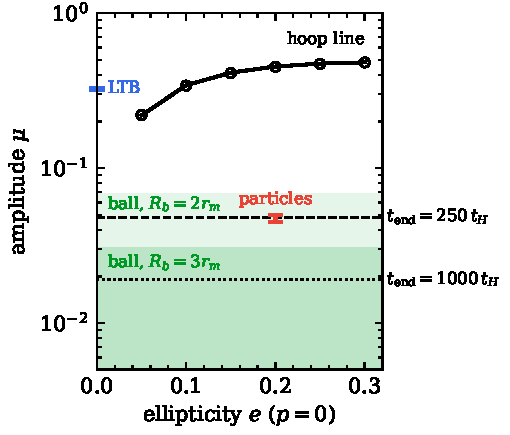
\includegraphics[width=\columnwidth]{fig_landscape.pdf}
\caption{The threshold plane. Line: the Zel'dovich-hoop line; circles: read off Ref.~\cite{Yoo:2026mdpbh}. Red and blue bars: the particle bracket of that work at $e=0.2$ and its exact-dust bracket. Dashed, dotted: amplitudes whose top-hat collapse time is $t_{\rm end}$. Green: what the ball holds at $R_bH_i=0.9$.}
\label{fig:landscape}
\end{figure}

The particle result of Ref.~\cite{Yoo:2026mdpbh} sits an order of magnitude below the hoop line and next to the amplitude whose top-hat collapse time equals the length of its runs. Four hypotheses could explain the low particle threshold, and each is decided by runs of its own. In H1 the threshold is set by the run length: the collapse time grows as $\mu^{-3/2}$, and the read-off collapse times of its particle runs follow the top-hat time of the compaction shell; H1 predicts horizons at the next lower amplitudes after longer runs. In H2 the black holes below the hoop line are produced by the violation of the Hamiltonian constraint where particles cross, which that work reports; a physical outcome is unchanged when constraint damping is switched off or the cell size halved. In H3 a cell-sized particle cloud smooths a pancake that would halt if its thickness were resolved; the three-way convergence of one outcome below the hoop line decides it. In H4 a spherical peak forms a black hole after the central shell crossing only near unit contrast \cite{Ebrahimian:2025md}, against the exact-dust bracket of Ref.~\cite{Yoo:2026mdpbh}; spherical particle runs continued past the crossing decide it.

\begin{figure}[t]
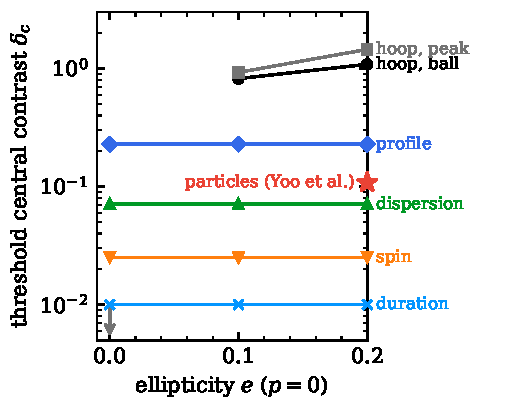
\includegraphics[width=\columnwidth]{fig_criteria.pdf}
\caption{Thresholds of six analytic criteria in the central contrast at horizon entry, at three ellipticities, for $\sigma_H=0.01$ and a matter era lasting to $a_{\rm end}/a_H=100$. Arrows: a vanishing threshold. Star: the particle result of Ref.~\cite{Yoo:2026mdpbh} in the same measure.}
\label{fig:criteria}
\end{figure}

The analytic criteria disagree in size and in their dependence on shape (Fig.~\ref{fig:criteria}). The two hoop criteria vanish for a spherical peak and rise steeply with the ellipticity; the spin, dispersion, profile and duration criteria are independent of the ellipticity, and at the comparison ellipticity the six criteria together span two orders of magnitude. At the comparison ellipticity the particle result lies between the profile criterion and the dispersion criterion, an order of magnitude below the hoop criteria. The predictions of all criteria for one parameter set form the prediction table against which the runs are compared item by item.

\section{Initial data and evolution}\label{sec:setup}

\subsection{The expanding ball}\label{sec:ball}

The verification set-up is a ball of collisionless matter that expands with the Hubble flow in vacuum. Its interior is exactly a Lema\^itre--Tolman--Bondi (LTB) dust solution until shells cross, and its exterior is Schwarzschild. On the slice of constant proper time $\tau$ of the matter, with the areal radius $R$ as coordinate,
\begin{equation}\label{eq:ltb}
\dd s^2 = -\dd\tau^2 + \frac{(\dd R - v\,\dd\tau)^2}{1+2E} + R^2\dd\Omega^2,\qquad v^2 = \frac{2m}{R}+2E,
\end{equation}
where $m(R)$ is the Misner--Sharp mass inside $R$, $E(R)$ the binding energy per unit mass of a shell, and $v=\dd R/\dd\tau$ its velocity. The lapse is one and the matter is at rest with respect to the normal observers. The extrinsic curvature follows from the change of the spatial metric between slices,
\begin{equation}\label{eq:kij}
K^R{}_R = -\frac{\dd v}{\dd R},\qquad K^\theta{}_\theta = K^\phi{}_\phi = -\frac{v}{R},
\end{equation}
with $K<0$ for expansion. With the scalar curvature of the slice, $-4(RE)'/R^2$, the Hamiltonian constraint becomes
\begin{equation}\label{eq:ham}
{}^{(3)}\!R + K^2 - K_{ij}K^{ij} = \frac{4m'}{R^2} = 16\pi\rho,
\end{equation}
the definition of the Misner--Sharp mass, and the momentum constraint, $\partial_R K^\theta{}_\theta = (K^R{}_R-K^\theta{}_\theta)/R$, holds identically. The data are therefore exact for any choice of $m(R)$ and $E(R)$.

The marginally bound ball, $E=0$, has a flat slice. Inside, $v=HR$ gives $K_{ij}=-H\gamma_{ij}$ and the Friedmann equation $8\pi\rho=3H^2$, so a ball of radius $R_b$ and mass $M$ obeys
\begin{equation}\label{eq:ballcondition}
\frac{2M}{R_b} = (HR_b)^2 .
\end{equation}
Outside, $v=\sqrt{2M/R}$ is the outgoing Painlev\'e--Gullstrand slice of Schwarzschild. The null expansions of a round sphere are $\theta_\pm=(2/R)(v\pm\sqrt{1+2E})$, so their product is $(4/R^2)(2m/R-1)$, and the slice holds an anti-trapped sphere only where $2m/R$ reaches one. By the ball condition above, a ball smaller than its Hubble radius starts free of anti-trapped spheres. These are the two relations of the program's brief marked for checking; both hold.

Turnaround and collapse need bound shells. The scouting data have a homogeneous bound core of mean contrast $\Delta$ inside the Einstein--de Sitter envelope, with $m(R)=\tfrac12H^2R^3(1+\Delta)$, a common bang time for every shell, which keeps the data in the growing mode, and a smooth step that compensates the core so that the envelope stays exactly Einstein--de Sitter and the exterior exactly Schwarzschild. A smooth taper at the surface removes the jump of $K^R{}_R$ that a sharp edge carries. Each shell then moves on its cycloid,
\begin{equation}\label{eq:cycloid}
R = \frac{m}{-2E}\,(1-\cos\eta),\qquad t = \frac{m}{(-2E)^{3/2}}\,(\eta-\sin\eta),
\end{equation}
with $t$ the time since the bang: it turns around at $\eta=\pi$, is trapped where $R=2m$, that is at $\cos\eta=1+4E$, and crunches at $\eta=2\pi$. A homogeneous core turns around and crunches as a whole, and its outermost shells are trapped first, as in Oppenheimer--Snyder collapse. These times are invariants, proper times along the matter between the initial slice and events defined by round spheres, so they can be compared with any slicing of the evolution through the proper time of the particles. The parameters of the scouting data are in Table~\ref{tab:parameters}.

The ball condition limits what the ball can hold. A ball of a few compaction radii has to be smaller than its Hubble radius, so it starts long after horizon entry, when the perturbation has grown. With the contrast at the start kept in the linear regime, a ball of three compaction radii holds amplitudes below the particle bracket of Ref.~\cite{Yoo:2026mdpbh}, a ball of two compaction radii reaches that bracket with the profile cut at its surface, and both stay an order of magnitude below the hoop line (Fig.~\ref{fig:landscape}). The ball is therefore the spherical verification case and the set-up for isolated collapses, and the threshold line is built in the periodic box.

\subsection{The periodic box}\label{sec:box}

The comparison set-up uses the initial data of Ref.~\cite{Yoo:2026mdpbh}: the long-wavelength growing mode of the curvature peak above on a slice of constant mean curvature, with the energy and momentum densities of the matter fixed by the constraints, in a periodic box several times the compaction radius, starting well before horizon entry. The matter is sampled on a lattice, either with masses that carry the density, as in that work, or with equal masses displaced by the growing-mode field. The box holds every amplitude of that work and is the set of the threshold line.

\subsection{Numerical methods}\label{sec:methods}

The evolution uses the Z4c formulation with particle-in-cell matter \cite{Wu:2026nrpic}: macroparticles move on geodesics with an implicit-midpoint or a spacetime Boris pusher, their energy, momentum and stress are deposited on the mesh with clouds of second to fourth order, and the metric is interpolated back to the particles. The ball enters as radial tables of the conformal factor, the extrinsic curvature, the lapse and the shift, with the particles on a lattice whose sites coincide with the cell centres. Two slicings are planned for the ball. Geodesic slicing keeps the lapse at one and the shift at zero, so the coordinates stay comoving and the coordinate time equals the proper time of every particle; the coordinate speed of light then grows inside the collapsing core, and the time step has to shrink in stages near the crunch. Conformal-time slicing, $\partial_t\alpha=-\tfrac13\alpha^2K$, keeps the coordinate speed of light near one; in the homogeneous core the lapse follows the scale factor of the core. An apparent-horizon finder gives the area mass of each horizon. The same particles also run under a Newtonian reference gravity, which serves the Newtonian precursor scan. Figure~\ref{fig:architecture} shows which parts of the calculation exist, which are carried over from another setting, and which are new.

\begin{figure*}[t]
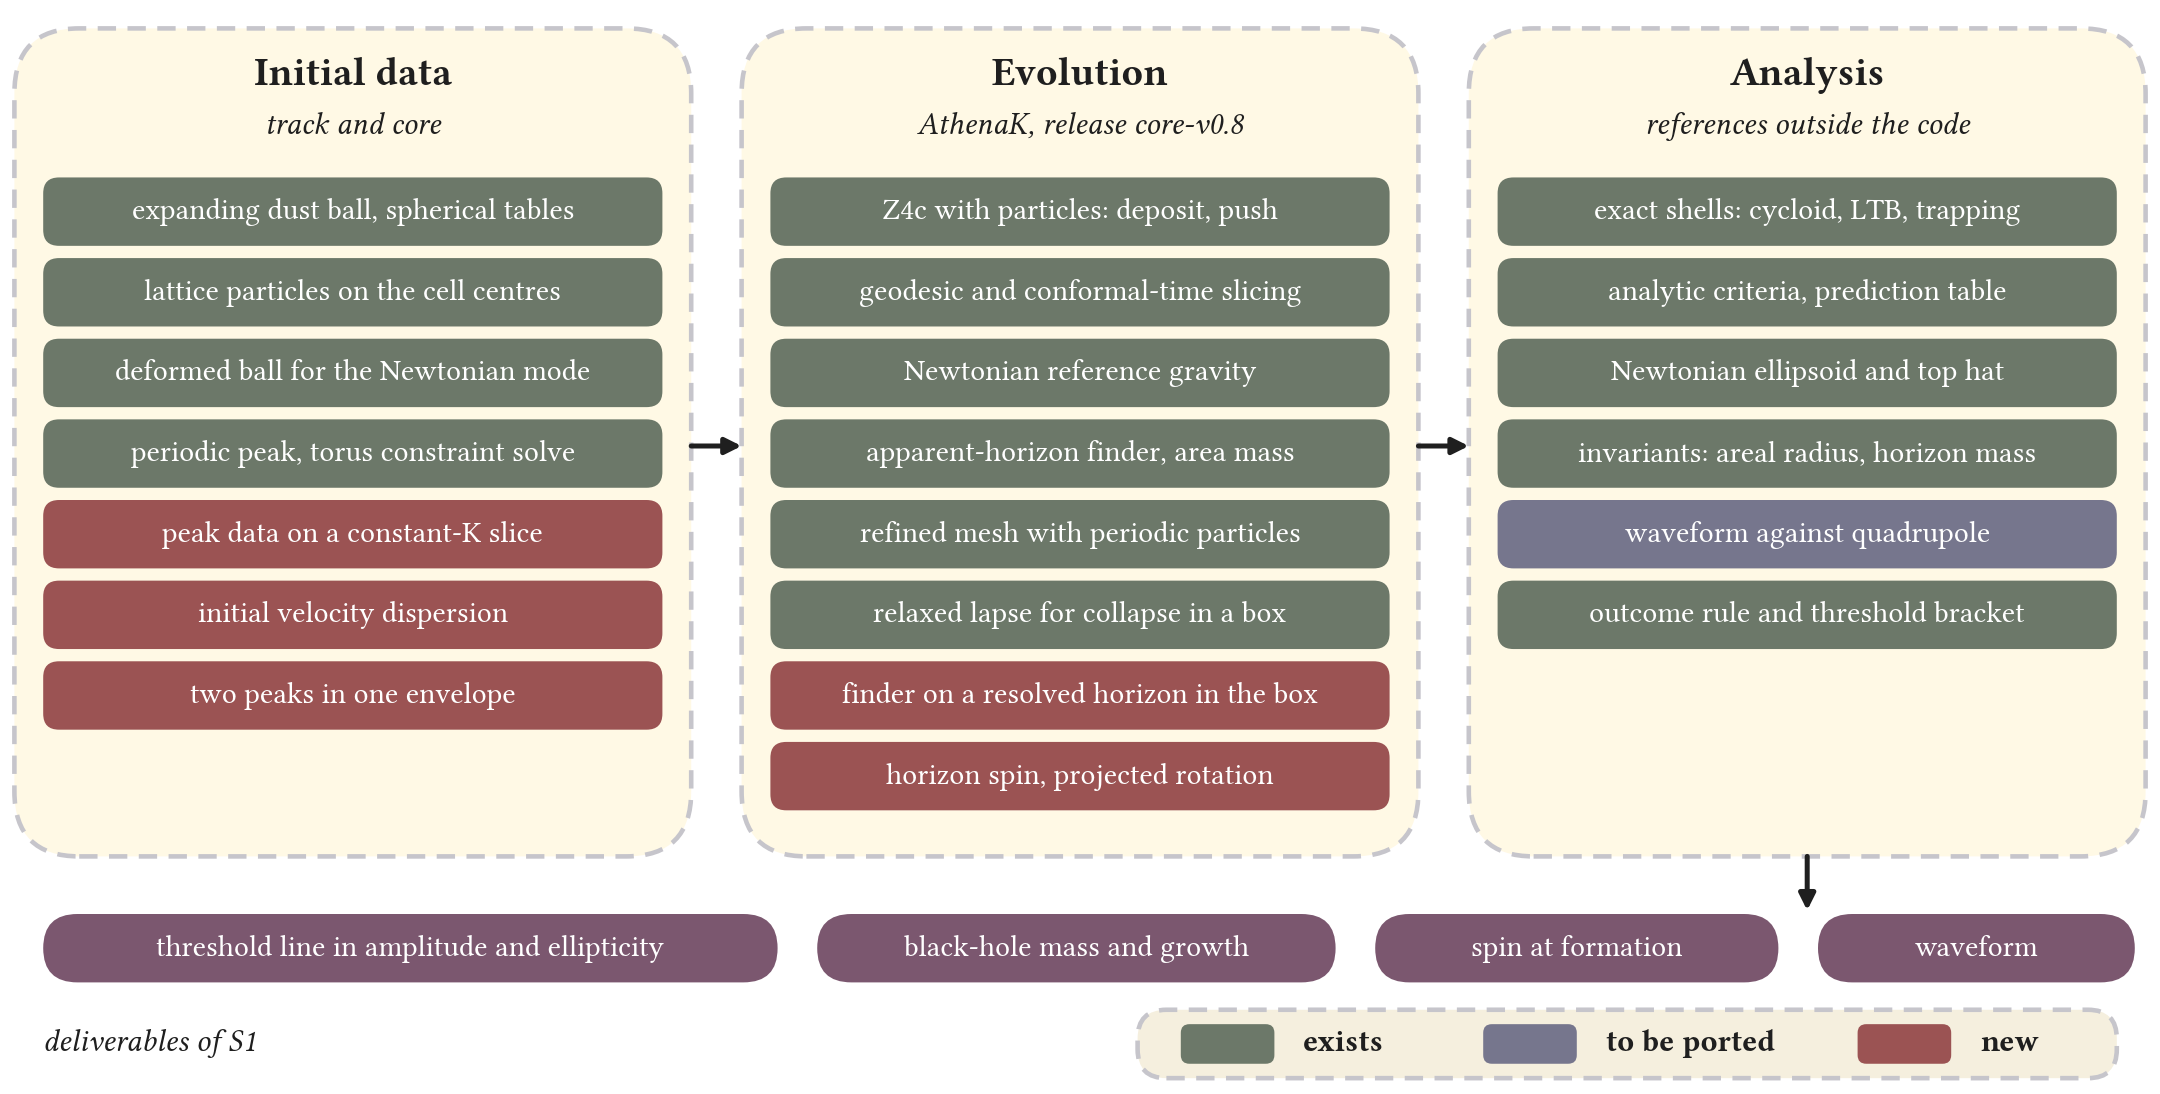
\includegraphics[width=\textwidth]{schem_architecture.png}
\caption{Architecture of the calculation. Initial data feed the evolution in AthenaK, whose output is compared with exact and semi-analytic references. Green: exists; slate: exists for another setting and is carried over; red: new. Bottom: the deliverables.}
\label{fig:architecture}
\end{figure*}

\section{Tests of the set-up}\label{sec:tests}

\subsection{Constraints of the initial data}\label{sec:constraints}

The initial data were checked offline on nested Cartesian meshes, with the Hamiltonian and momentum constraints evaluated by finite differences of second and fourth order. Smooth data converge at the order of the differences (Fig.~\ref{fig:constraints}): the momentum constraint of the marginally bound ball with a tapered edge and both constraints of the smoothed top-hat core approach fourth order on the finest meshes, and the compensated top hat converges at fourth order away from its edges. Over all cells a sharp edge leaves a residual band one cell wide whose norm grows as the cells shrink. Every evolution therefore starts from tapered data; sharp data serve offline tests only.

\begin{figure*}[t]
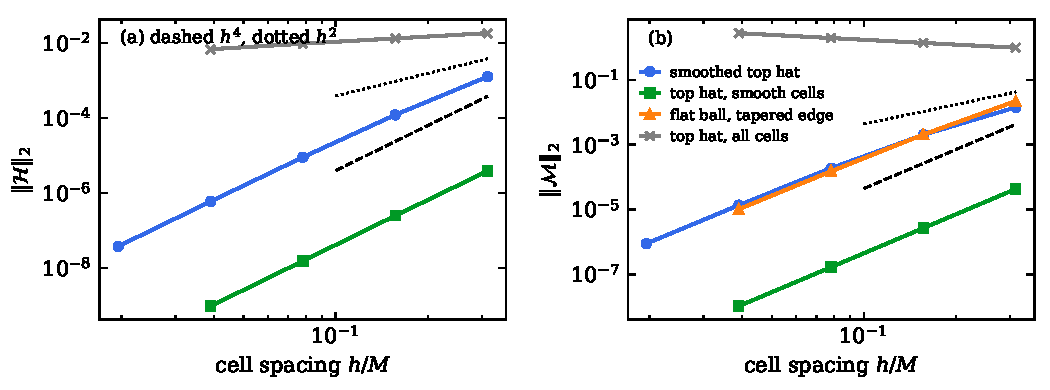
\includegraphics[width=\textwidth]{fig_constraints.pdf}
\caption{Norms of the Hamiltonian (a) and momentum (b) constraint residuals of the initial data against cell spacing, with fourth-order differences. Smooth cells exclude a band around radii where the data have a jump. Dashed and dotted: slopes four and two. The flat ball satisfies the Hamiltonian constraint to rounding error and appears in (b) only.}
\label{fig:constraints}
\end{figure*}

\subsection{Exact evolution of the scouting data}\label{sec:exact}

The exact solution of the scouting data gives the predictions of the first runs (Fig.~\ref{fig:ball}). The core expands, turns around and crunches, while the envelope expands for ever. The first trapped sphere appears just outside the edge of the homogeneous core, in the smooth step, shortly before the crunch; the core edge is trapped after it, and the horizon mass grows steeply over the remaining time to the crunch. In geodesic slicing the largest coordinate speed of light stays of order one until late in the collapse and then grows without bound, so the time step is halved in stages, each stage ending where the speed reaches the stability bound of the discretization. In conformal-time slicing the same events fall at other coordinate times, earlier for the turnaround and later for trapping and crunch, with the coordinate speed of light near one throughout. The predicted times, and what would refute each prediction, were written into the track's journal before any run.

\begin{figure*}[t]
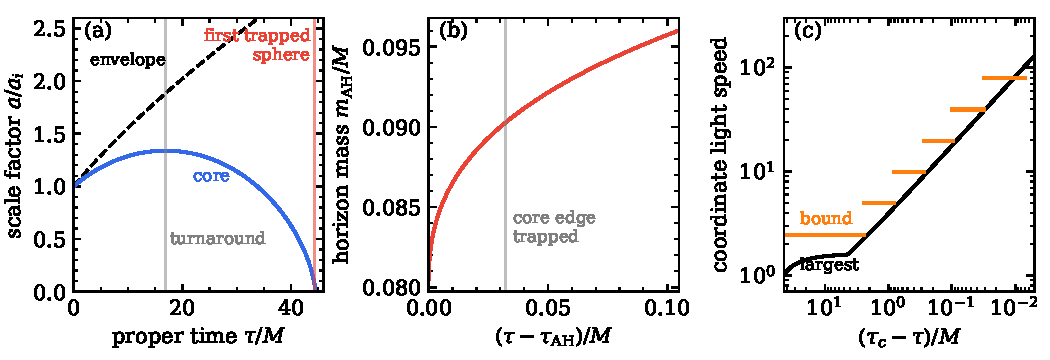
\includegraphics[width=\textwidth]{fig_ball_exact.pdf}
\caption{Exact evolution of the scouting data. (a) Scale factor of the bound core (blue) and of the expanding envelope (dashed) against proper time; vertical lines: turnaround and first trapped sphere. (b) Mass of the outermost trapped sphere after the first one appears. (c) Largest coordinate speed of light in geodesic slicing (black) and the stability bound of each stage of the time step (orange), against the time left to the crunch.}
\label{fig:ball}
\end{figure*}

\subsection{Independent re-derivations}\label{sec:rederivations}

Every result of the scoping stage was recomputed by a second agent from the committed scripts and reproduced to the last printed digit. Two constructions of the ball data written independently, one for the track and one inside the code project, agree to rounding error, and so do the two readers of the radial tables. The turnaround, trapping and crunch times of a bound test ball agree to rounding error between three independent codes, one of them the closed-form cycloid. On the exterior slice the trace of the extrinsic curvature equals the Painlev\'e--Gullstrand value to rounding error, and it halves across a sharp surface, as the extrinsic curvature above requires.

\subsection{Analytic criteria against their papers}\label{sec:criteria}

The criteria of Fig.~\ref{fig:criteria} were coded from five papers, each function with the line of the formula it implements, and checked against values and curves printed in those papers. All but four checks pass; two of the four differ in the last printed digit of the paper, and two compare quantities whose agreement band was set too tight. The checks, the failures and their reasons are on record.

\section{Plan to the next gates}\label{sec:plan}

The test plan holds the rows of the program's verification suite owned by this track: the time reverse of Oppenheimer--Snyder collapse, run as the expanding ball with a bound core; oblate and prolate collapse with the first caustic against the Zel'dovich time; the LTB dust profile of Ref.~\cite{Yoo:2026mdpbh} against its exact solution; quasi-spherical Szekeres dust; and three track tests, the hoop line, the halting references of the Newtonian mode, and the hypotheses H1--H4. The gate of verified capability asks that in the spherical case the errors of the turnaround and horizon-formation times converge in particle number, cell size and ball radius, and that the horizon-mass error be of the same order as in the Oppenheimer--Snyder test of Ref.~\cite{Wu:2026nrpic}. The gate of science runs asks for the converged threshold line at five ellipticities, the four hypotheses decided, mass and spin at formation and after accretion, and one waveform against the quadrupole estimate of Ref.~\cite{Escriva:2026gw}. Figure~\ref{fig:timeline} places the gates in time.

\begin{figure*}[t]
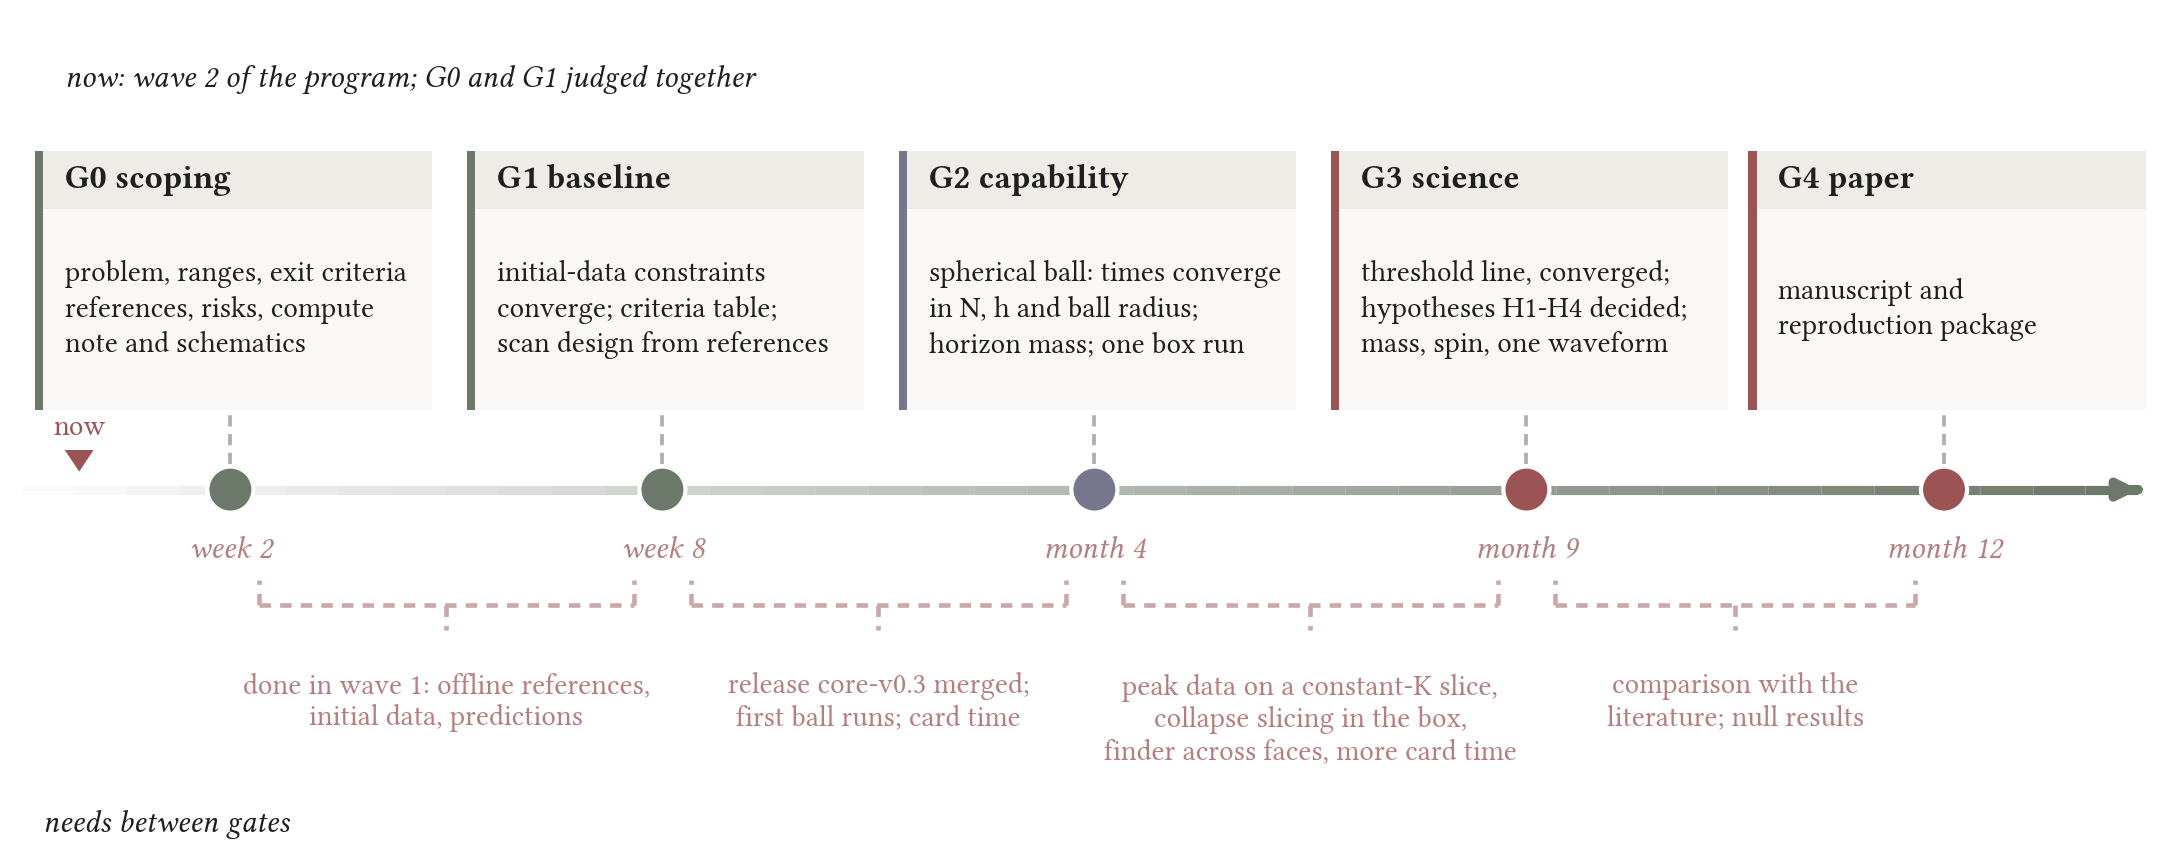
\includegraphics[width=\textwidth]{schem_timeline.png}
\caption{Stage timeline of the track. Circles: the five gates at the target times of the program (green: scoping and baseline; slate: verified capability; red: science and paper). Boxes: what each gate requires. Dashed brackets: what the step between two gates needs.}
\label{fig:timeline}
\end{figure*}

The first two runs in full general relativity evolve the scouting data in geodesic and in conformal-time slicing. A first attempt at the coarser resolution was stopped after a few steps as too slow for the time available, with its cause on record; both runs are now queued at the coarser resolution, and the finer one follows. The first tests in the periodic box found that a static refined mesh keeps a homogeneous universe homogeneous to rounding error when the particle clouds are deposited at one common level, and that the horizon finder recovers the mass of a calibrated vacuum black hole in a periodic box; they also found that the finder searches only inside the box, so a peak has to sit at the box centre, and that adaptive refinement with periodic particles stopped at its first refinement check, which is being repeated. The Newtonian mode of the code now exists, and the first Newtonian runs of the top hat and the deformed ball are under way.

Open at this stage: the key statements of the references are verified at their sources and wait to enter the knowledge base; four references of the test plan are still unread, among them the Szekeres solutions; the conversion between the two amplitude measures is being added to the prediction table; and the threshold line needs, from the code project, the peak data on a slice of constant mean curvature, a slicing that survives collapse in a periodic box, the finder across the box faces and the spin of a horizon in an expanding region, and from the computing allotment a raise once the verified-capability gate is passed.

\section{Summary}\label{sec:summary}

The threshold for black holes in an early matter era is set by whatever halts a collapse first, so it depends on shape, dispersion, spin and the duration of the era; its definition for collisionless matter therefore names the run length and the cutoff that length implies. The one particle calculation in full general relativity sits an order of magnitude below the hoop estimate and next to the finite-duration amplitude of its own run length, and four hypotheses, each with a decisive run, account for the difference. The expanding ball is exact before shells cross and serves verification; its Hubble-radius condition keeps the comparison amplitudes out of reach, so the threshold line is built in a periodic box. The initial data, their exact evolution and the analytic criteria are verified offline and by independent recomputation, and the first runs in full general relativity carry written predictions.

\begin{acknowledgments}
The calculations, the code and this note were produced by large-language-model agents under human direction, within the numerical-relativity particle-in-cell cosmology program.
\end{acknowledgments}

\appendix

\section{Parameters}\label{app:parameters}

Table~\ref{tab:parameters} lists the parameters of the scouting data and the constants of the outcome rule.

% generated from registered run outputs; do not edit
\begin{table*}
\caption{Parameters of the scouting data and of the outcome rule.}
\label{tab:parameters}
\begin{ruledtabular}
\begin{tabular}{p{0.62\textwidth}l}
\multicolumn{2}{l}{\emph{Scouting data: expanding ball with a bound core}} \\
total (Misner--Sharp) mass $M$; rest mass & 1.0096; 1.0159 \\
envelope: $HR_b$; ball radius $R_b/M$; Hubble rate $HM$; start $t_i/M$ & 0.5; 8; 0.0625; 10.667 \\
core: mean contrast $\Delta$ inside $R/M$; compensated at $R/M$ & 1; 2.4; 6 \\
edge taper: half width$/M$; matter edge$/M$ & 1.5; 9.5 \\
conformal factor at the centre; largest $2m/R$ on the slice & 1.0138; 0.236 \\
particle lattice spacing$/M$ & 0.5 \\
\multicolumn{2}{l}{\emph{Outcome rule and threshold bracket (design)}} \\
consecutive horizon searches; their span in units of the horizon mass & 3; 5 \\
constraint bound: $\|\Ham\|_2$ over $\|16\pi E\|_2$ outside the horizon & 0.1 \\
bracket ratio $A_{\rm hi}/A_{\rm lo}$ at the end of the bisection & 1.1 \\
primary end time; continuation of the run below threshold ($t_H$) & 250; 1000 \\
\end{tabular}
\end{ruledtabular}
\end{table*}


\section{Numerical ledger}\label{app:ledger}

Table~\ref{tab:ledger} gives every number behind this note with the registered run that produced it; the outputs of each run are checked against the checksums the run recorded. The amplitudes of Ref.~\cite{Yoo:2026mdpbh} come from its source, \texttt{MDPBH.tex} lines 1101--1103 (particle bracket at $e=0.2$), 765--768 (exact-dust bracket), 907--908 and 918 (deformation eigenvalues and hoop function); the horizon-mass error of the Oppenheimer--Snyder test of Ref.~\cite{Wu:2026nrpic} from its source, \texttt{main.tex} lines 945 and 1484. The statements of Sec.~\ref{sec:plan} about the runs under way come from runs A-emd-pbh-20261115-153856-9d731b1 and -153903-9d731b1 (processor attempt), A-emd-pbh-20261115-155056-ec1b816 (submitted) and A-emd-pbh-20261115-154250-527a6d1 (periodic box tests), as recorded in the journals of the track. The figures and tables were made from these runs in run A-20261115-161720-6ae975e. % generated; do not edit
A check of 68 numbers stated in the track's status documents and journals against the run outputs found 66 in agreement and two differences%: a bound printed as an upper limit that the value exceeds in its third digit, and an edge deviation of the table interpolation described as an overshoot of a tenth of the Hubble rate where the recorded largest deviation, which contains the smeared jump, is larger than the Hubble rate.

% generated from registered run outputs; do not edit
\begin{table*}
\caption{Numerical ledger. Every number of this note with the registered run that produced it: scoping and offline tests.}
\label{tab:ledger}
\begin{ruledtabular}
\begin{tabular}{p{0.44\textwidth}p{0.22\textwidth}l}
Quantity & Value & Run \\
\hline
\multicolumn{3}{l}{\emph{Threshold landscape}} \\
Zel'dovich-hoop amplitude $\hat h(0.2,0)$ & 0.452 & \texttt{\footnotesize A-20261115-130252-7877b7a} \\
largest deviation of $\hat h$ from the values read off Ref.~\cite{Yoo:2026mdpbh} & 0.0025 & \texttt{\footnotesize A-20261115-130252-7877b7a} \\
top-hat amplitude $\mu_{\rm fd}$ for $t_{\rm end}=100,250,400,1000\,t_H$ & 0.089, 0.048, 0.035, 0.019 & \texttt{\footnotesize A-20261115-130252-7877b7a} \\
slope of the read-off collapse times against $\mu$ & -1.31 & \texttt{\footnotesize A-20261115-130252-7877b7a} \\
read-off collapse time over top-hat time at $r_m$, $\mu\le0.15$ (range; median); median over all six read-offs & 0.80--1.01; 0.84; 0.86 & \texttt{\footnotesize A-20261115-130252-7877b7a} \\
largest $\mu$ in the ball, $R_bH_i=0.9$, $R_b=2,3,4\,r_m$ (mean contrast $0.3$) & 0.069, 0.031, 0.017 & \texttt{\footnotesize A-20261115-130252-7877b7a} \\
the same with the central contrast at most $0.3$ & 0.0253, 0.0113, 0.0063 & \texttt{\footnotesize A-20261115-130252-7877b7a} \\
critical dispersion $s$: virial halt; crossing time & 0.55; 1.5 & \texttt{\footnotesize A-20261115-130252-7877b7a} \\
measured cost of the two-overdensity run (card-hours; s per cycle) & 5.41; 0.761 & \texttt{\footnotesize A-20261115-130252-7877b7a} \\
modelled cost per run (range; median at $10^6$ particles), card-hours & 1.1--3.5; 2.4 & \texttt{\footnotesize A-20261115-130252-7877b7a} \\
first scan: runs; card-hours & 65; 155 & \texttt{\footnotesize A-20261115-130252-7877b7a} \\
\multicolumn{3}{l}{\emph{Analytic criteria}} \\
threshold $\delta_c$ at $e=0.2$: hoop (ball); hoop (peak); profile; dispersion; spin; duration & 1.08; 1.45; 0.229; 0.0712; 0.0252; 0.01 & \texttt{\footnotesize A-emd-pbh-20261115-120425-80492f8} \\
particle threshold of Ref.~\cite{Yoo:2026mdpbh} in the same measure & 0.108 & \texttt{\footnotesize A-emd-pbh-20261115-120425-80492f8} \\
first check run against the five papers: passed of total; failing & 33 of 37; T1.2b, T2.2d, T2.4a, T2.4c & \texttt{\footnotesize A-emd-pbh-20261115-130256-a7374a4} \\
checks of the hoop, dispersion, profile and peak criteria: passed of total; kept as diagnostics & 24 of 24; 1 & \texttt{\footnotesize A-emd-pbh-20261115-161813-6c820fb} \\
checks of the spin and duration criteria: passed of total; kept as diagnostics & 17 of 17; 3 & \texttt{\footnotesize A-emd-pbh-20261115-163358-9b2d048} \\
\multicolumn{3}{l}{\emph{Initial data}} \\
order of $\|\mathcal M\|_2$, flat ball, smooth cells, differences of order 2; 4 & 2.00; 4.00 & \texttt{\footnotesize A-emd-pbh-20261115-130402-f5566fb} \\
order of $\|\mathcal M\|_2$, tapered edge, all cells, order 2; 4 & 1.99; 3.90 & \texttt{\footnotesize A-emd-pbh-20261115-130402-f5566fb} \\
order of $\|\mathcal H\|_2$; $\|\mathcal M\|_2$, top hat, smooth cells, order 4 & 4.00; 4.00 & \texttt{\footnotesize A-emd-pbh-20261115-130402-f5566fb} \\
order of $\|\mathcal M\|_2$, top hat, all cells, order 4 & -0.50 & \texttt{\footnotesize A-emd-pbh-20261115-130402-f5566fb} \\
order of $\|\mathcal H\|_2$; $\|\mathcal M\|_2$, smoothed top hat, $N=256\to512$ & 3.98; 3.94 & \texttt{\footnotesize A-emd-pbh-20261115-122117-aa1c84d} \\
largest difference of two independent generators (flat ball) & 4.8e-15 & \texttt{\footnotesize A-20261115-130257-a7374a4} \\
largest difference of two table evaluators & 6.9e-18 & \texttt{\footnotesize A-20261115-130257-a7374a4} \\
largest difference of three exact-solution codes (times) & 1.1e-14 & \texttt{\footnotesize A-20261115-130257-a7374a4} \\
exterior $K$ against $-\tfrac32\sqrt{2M/R^3}$, largest relative difference & 4.3e-15 & \texttt{\footnotesize A-20261115-130257-a7374a4} \\
\end{tabular}
\end{ruledtabular}
\end{table*}

\begin{table*}
\caption{Numerical ledger (continued): exact solution and Newtonian limit.}
\label{tab:ledger2}
\begin{ruledtabular}
\begin{tabular}{p{0.44\textwidth}p{0.22\textwidth}l}
Quantity & Value & Run \\
\hline
\multicolumn{3}{l}{\emph{Exact solution of the scouting data}} \\
total mass $M/M_0$; rest mass$/M_0$ & 1.00959; 1.01590 & \texttt{\footnotesize A-emd-pbh-20261115-153719-91b03d1} \\
core turnaround $\tau_{\rm ta}/M_0$; $R_{\max}/R_i$ & 16.894; 1.3398 & \texttt{\footnotesize A-emd-pbh-20261115-153719-91b03d1} \\
first trapped sphere $\tau_{\rm AH}/M_0$; shell $R_i/M_0$; $m_{\rm AH}/M_0$; areal radius$/M_0$ & 44.349; 2.742; 0.0805; 0.161 & \texttt{\footnotesize A-emd-pbh-20261115-153719-91b03d1} \\
core edge trapped; crunch of the core ($\tau/M_0$) & 44.381; 44.454 & \texttt{\footnotesize A-emd-pbh-20261115-153719-91b03d1} \\
$m_{\rm AH}/M_0$ at the crunch & 0.0960 & \texttt{\footnotesize A-emd-pbh-20261115-153719-91b03d1} \\
in units of the total mass: $\tau_{\rm ta}/M$; $m_{\rm AH}/M$ at first trapping and at the crunch & 16.73; 0.0797; 0.0951 & \texttt{\footnotesize A-emd-pbh-20261115-153719-91b03d1} \\
conformal-time coordinate times: turnaround, core at $\tau_{\rm AH}$, crunch & 13.82, 49.51, 54.96 & \texttt{\footnotesize A-20261115-130948-5a2b58a} \\
geodesic slicing reaches the step bound at ${\rm cfl}=0.25$ ($\tau/M_0$; light speed $R_i/R$, without the conformal factor) & 42.30 & \texttt{\footnotesize A-20261115-130948-5a2b58a} \\
predicted card-hours of the two scouting runs & 0.15; 0.16 & \texttt{\footnotesize A-20261115-130948-5a2b58a} \\
\multicolumn{3}{l}{\emph{Newtonian limit}} \\
top hat, $128^3$ cells, $2.7\times10^5$ particles: relative error of the turnaround time; largest radius; time at a quarter of it; softened collapse & +7.2e-4; +4.3e-4; +8.4e-4; +2.6e-4 & \texttt{\footnotesize A-emd-pbh-20261115-164420-4528861} \\
the same four errors: reduction per doubling of the mesh, $32^3\to64^3\to128^3$ (range) & 4.0--6.1 & \texttt{\footnotesize A-emd-pbh-20261115-164420-4528861} \\
top hat, $128^3$: largest relative energy error & 9.5e-5 & \texttt{\footnotesize A-emd-pbh-20261115-164420-4528861} \\
first collapse against the homogeneous ellipsoid, the 9 points at $128^3$ with at least $2.7\times10^5$ particles other than the spindle: relative error of $t_1$ (range); of the hoop ratio (largest) & +2.2e-4 to +6.3e-4; 6.1e-4 & \texttt{\footnotesize A-emd-pbh-20261115-164420-4528861} \\
scan points whose first collapse is along the predicted axis & 14 of 14 & \texttt{\footnotesize A-emd-pbh-20261115-164420-4528861} \\
the same for the spindle ($p=-e$); the $64^3$ controls; the $3.4\times10^4$-particle controls & +1.5e-3; +8.8e-4, +1.5e-3; -4.6e-4, -2.4e-4 & \texttt{\footnotesize A-emd-pbh-20261115-164420-4528861} \\
relative energy error to $0.9\,t_1$ (largest); at the first crossing (range); spindle & 1.9e-4; 1.1e-3 to 9.3e-3; 3.0e-2 & \texttt{\footnotesize A-emd-pbh-20261115-164420-4528861} \\
Newtonian hoop amplitude $\delta_{L,\rm th}$ at $e=0.05,0.1,0.2,0.3$ ($p=0$) & 0.359, 0.592, 0.854, 0.968 & \texttt{\footnotesize A-emd-pbh-20261115-164757-b8bc9a3} \\
\end{tabular}
\end{ruledtabular}
\end{table*}

\begin{table*}
\caption{Numerical ledger (continued): first evolutions in full general relativity.}
\label{tab:ledger3}
\begin{ruledtabular}
\begin{tabular}{p{0.44\textwidth}p{0.22\textwidth}l}
Quantity & Value & Run \\
\hline
\multicolumn{3}{l}{\emph{First evolutions of the scouting data}} \\
geodesic slicing, $\Delta x=M_0/2$: largest $|r/r_0-1|$ of the tracked particles; largest $|\tau-t|/M_0$ & 8.2e-15; 6.3e-12 & \texttt{\footnotesize A-emd-pbh-20261115-163659-4dbacd0} \\
core shells, largest $|R/R_{\rm exact}-1|$ at $\tau=16.9\,M_0$, geodesic slicing, $\Delta x=M_0,\,M_0/2,\,M_0/4$ (the last with half the box) & 5.6e-2, 6.2e-3, 7.6e-4 & \texttt{\footnotesize A-20261115-182657-53da696} \\
the same, conformal-time slicing & 2.1e-2, 7.5e-3, 3.7e-4 & \texttt{\footnotesize A-20261115-182657-53da696} \\
core turnaround, mean proper-time error$/M_0$, geodesic slicing, $\Delta x=M_0/2,\,M_0/4$ & -0.0224, -0.0125 & \texttt{\footnotesize A-20261115-182657-53da696} \\
the same, conformal-time slicing, from the vertex of three records of $R(\tau)$ (depends on the estimator) & +0.0434, +0.0308 & \texttt{\footnotesize A-20261115-182657-53da696} \\
geodesic slicing: largest $|\mathcal H|$ on the mesh at $t=20\,M_0$, $\Delta x=M_0,\,M_0/2,\,M_0/4$ & 0.24, 0.051, 0.04 & \texttt{\footnotesize A-20261115-182657-53da696} \\
geodesic slicing: first non-finite line output, $t/M_0$ at $\Delta x=M_0,\,M_0/2$ & 31; 33.25 & \texttt{\footnotesize A-emd-pbh-20261115-163659-4dbacd0} \\
conformal-time slicing: central lapse off the exact core value by more than a tenth from $t/M_0$, $\Delta x=M_0,\,M_0/2,\,M_0/4$ & 6.5, 6.625, 6.625 & \texttt{\footnotesize A-20261115-182657-53da696} \\
conformal-time slicing, $\Delta x=M_0/2$: largest relative departure of the central lapse from the scale factor of the core up to $t=15\,M_0$ & 0.39 & \texttt{\footnotesize A-emd-pbh-20261115-163659-4dbacd0} \\
conformal-time slicing, $\Delta x=M_0/2$: largest $2m/R$ on the axes; apparent horizons found & 0.34; 0 & \texttt{\footnotesize A-emd-pbh-20261115-163659-4dbacd0} \\
\multicolumn{3}{l}{\emph{Parameters}} \\
scouting data of Table~\ref{tab:parameters} & see table & \texttt{\footnotesize A-emd-pbh-20261115-130609-947c898} \\
\end{tabular}
\end{ruledtabular}
\end{table*}



\bibliography{references}

\end{document}
